\begin{center}
\large\noindent\fbox{
	\parbox{\textwidth}{
	Utilizzare le functions degli esercizi precedenti per disegnare l'approssimazione della funzione \(\sin(x)\) nell'intervallo \([0, 2\pi]\), utilizzando le ascisse di interpolazione \(x_i=i\pi\), \(i= 0,1,2\).
	}
}\end{center}

\noindent Il seguente codice Matlab contiene le chiamate alle funzioni degli esercizi precedenti: \\ \textit{y = newton(xi, fi, x)}; \\ \textit{y = lagrange(xi, fi, x)}; \\ \textit{y = hermite(xi, fi, f1i, x)}; \\ 
calcolate fornendo in input le ascisse \(0, \pi, 2\pi \) e la loro immagine attraverso \(f\)=\(\sin(x)\). Nel caso di Hermite anche la loro immagine attraverso \(f'\)=\(\cos(x)\).

\lstinputlisting[language=Matlab]{Codici/Cap4/Es4_Cap4.m}

\pagebreak
\noindent Nella figura sottostante \'e riportata l'approssimazione della funzione \(\sin(x)\) tramite l'utilizzo delle funzioni di interpolazione:\\

\begin{figure}[H]
	\centering
	\label{Cap4_Es_4}
	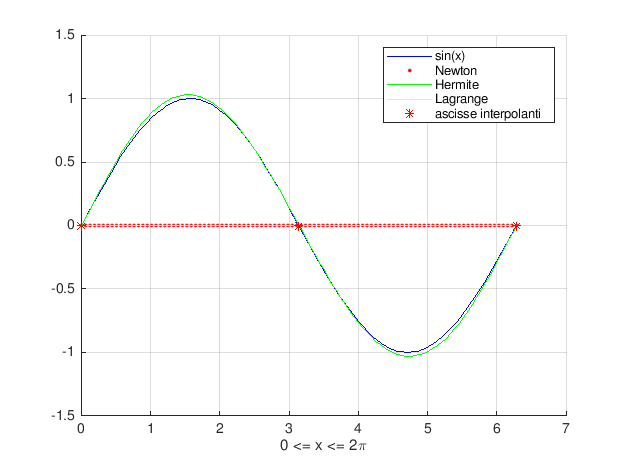
\includegraphics[width=\textwidth,height=\textheight,keepaspectratio]{Codici/Cap4/es4_cap4.png}
\end{figure}

\noindent Essendo \(f_i=0\) per tutte le ascisse \(x_i\), sia il polinomio interpolante di Lagrange, che quello di Newton in realt\'a sono la retta \(y=0\). \\ \\